% generado por el cuaderno homónimo; no editar
\begin{subfigure}[t]{0.32\textwidth}
    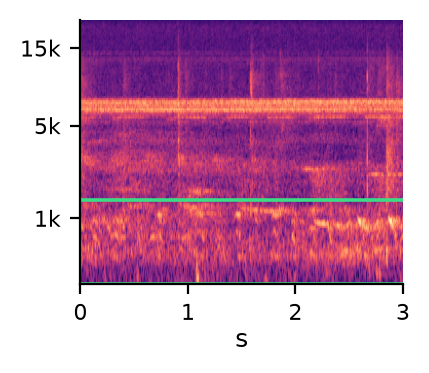
\includegraphics[width=\linewidth]{figures/RE_1-3/galeria_pt_dc}
    \caption{\code{pt/dc}, duet call, 6,7\,s}
\end{subfigure}\hfill
\begin{subfigure}[t]{0.32\textwidth}
    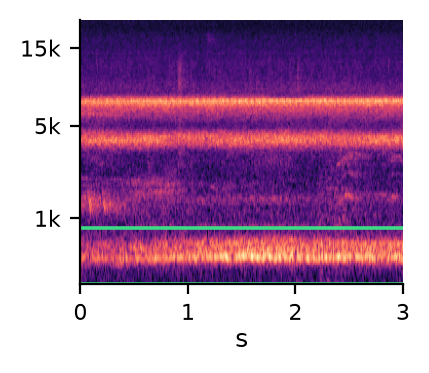
\includegraphics[width=\linewidth]{figures/RE_1-3/galeria_as_hc}
    \caption{\code{as/hc}, howl call, 11,0\,s}
\end{subfigure}\hfill
\begin{subfigure}[t]{0.32\textwidth}
    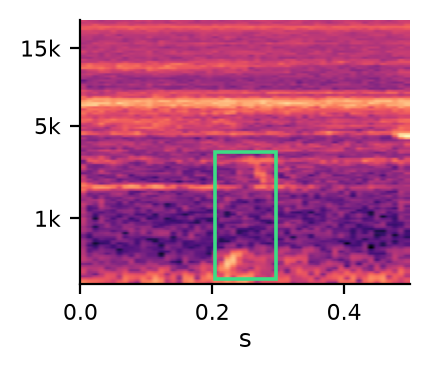
\includegraphics[width=\linewidth]{figures/RE_1-3/galeria_aa_gc}
    \caption{\code{aa/gc}, gulp call, 0,09\,s}
\end{subfigure}\\[1.5ex]
\begin{subfigure}[t]{0.32\textwidth}
    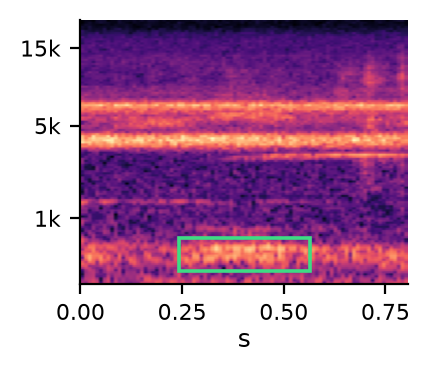
\includegraphics[width=\linewidth]{figures/RE_1-3/galeria_as_bc}
    \caption{\code{as/bc}, bark call, 0,32\,s}
\end{subfigure}\hfill
\begin{subfigure}[t]{0.32\textwidth}
    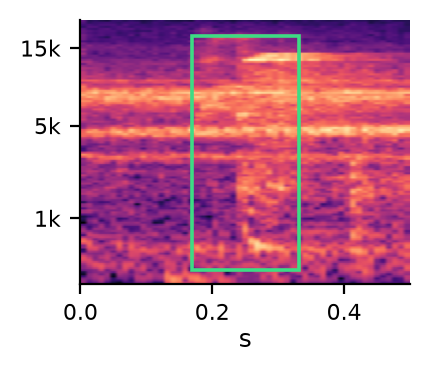
\includegraphics[width=\linewidth]{figures/RE_1-3/galeria_sb_spc}
    \caption{\code{sb/spc}, spit call, 0,16\,s}
\end{subfigure}\hfill
\begin{subfigure}[t]{0.32\textwidth}
    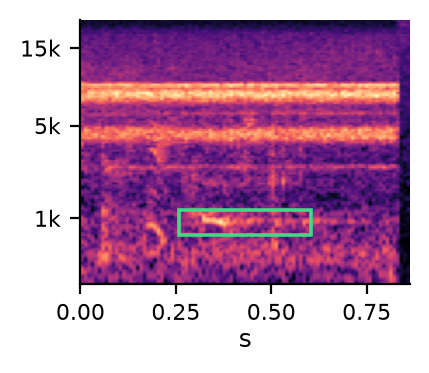
\includegraphics[width=\linewidth]{figures/RE_1-3/galeria_ac_bc}
    \caption{\code{ac/bc}, bark call, 0,35\,s}
\end{subfigure}\\[1.5ex]
\begin{subfigure}[t]{0.32\textwidth}
    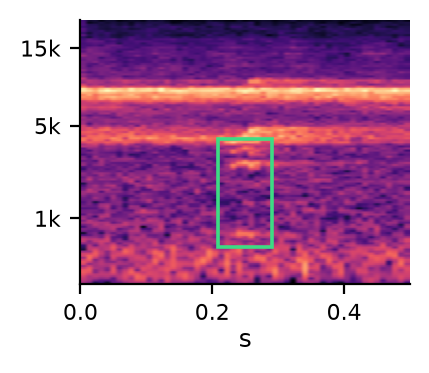
\includegraphics[width=\linewidth]{figures/RE_1-3/galeria_sm_cc}
    \caption{\code{sm/cc}, contact call, 0,08\,s}
\end{subfigure}\hfill
\begin{subfigure}[t]{0.32\textwidth}
    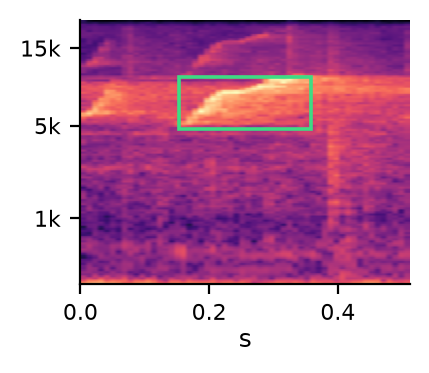
\includegraphics[width=\linewidth]{figures/RE_1-3/galeria_sb_ppc}
    \caption{\code{sb/ppc}, play peep call, 0,20\,s}
\end{subfigure}\hfill
\begin{subfigure}[t]{0.32\textwidth}
    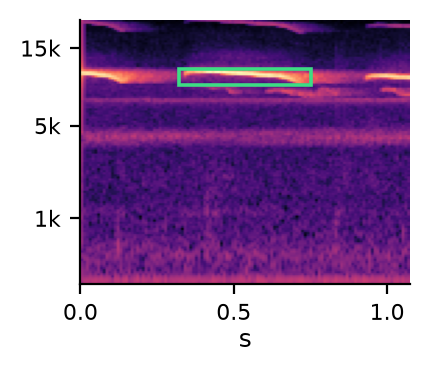
\includegraphics[width=\linewidth]{figures/RE_1-3/galeria_lw_cs}
    \caption{\code{lw/cs}, contact syllable, 0,43\,s}
\end{subfigure}
